\uuid{tCv2}
\exo7id{7283}
\titre{exo7 7283}
\auteur{mourougane}
\organisation{exo7}
\datecreate{2021-08-10}
\isIndication{false}
\isCorrection{false}
\chapitre{Géométrie affine euclidienne}
\sousChapitre{Géométrie affine euclidienne du plan}
\module{Géométrie}
\niveau{L2}
\difficulte{}

\contenu{
\texte{
Étant données deux longueurs \(a\) et \(b\), construire à la 
règle et au compas la longueur \(\sqrt{ab}\). (Indication: on pourra 
considérer la figure ci-dessous.)

Pourquoi, dans cet exercice et dans le précédent, a-t-on considéré 
les longueurs \(\frac{ab}{c}\) et \(\sqrt{ab}\) plutôt que \(ab\), 
\(\frac{a}{c}\) et \(\sqrt{a}\)?

\begin{center}
    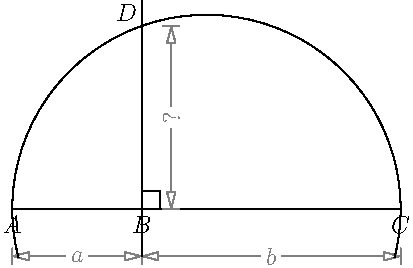
\includegraphics[scale=1]{images/pdf/tCv2-1.pdf}
\end{center}

% [[figure asymptote]]

%\begin{center}
%\begin{asy}
%size(7cm, 0);
%point A = (0, 0); label("\(A\)", A, S);
%point B = (1, 0); label("\(B\)", B, S);
%point C = (3, 0); label("\(C\)", C, S);
%line L0 = line(A, C);
%draw(A -- C);
%distance("\(a\)", A, B, 8mm, gray);
%distance("\(b\)", B, C, 8mm, gray);
%circle C0 = circle(A, C);
%line L1 = perpendicular(B, L0);
%point[] D = intersectionpoints(C0, L1);
%label("\(D\)", D[1], NW);
%draw(L1);
%perpendicularmark(L0, L1);
%distance("?", B, D[1], 5mm, gray);
%clipdraw(C0);
%\end{asy}
%\end{center}
}
}
